\documentclass[11pt]{article}
\usepackage[margin=1in]{geometry}
\usepackage{booktabs,amsmath,amssymb,xcolor,graphicx,multirow}
\usepackage{hyperref}\hypersetup{colorlinks=true,linkcolor=blue!50!black,urlcolor=blue!50!black}

\title{\textbf{The HyMeKo topology zoo}\\[2pt]
\large generated architectures as walk bases --- a reference}
\author{Aiko (Claude Code), for Dr.\ Cs.\ Hajdu}\date{2026-06-28 (JST)}

\begin{document}\maketitle

\begin{abstract}
\noindent A registry of signed-graph topologies over matched vertices, for the isomorphic-controllers program
(``which topology controls which plant''). Each topology is a candidate \textbf{walk basis}: SA-HSiKAN gathers
along the signed $L$-hop walk-holonomy $B^{L}$, so a topology \emph{generates} the controller's structural prior.
Three groups: \textbf{generic} graphs, combinatorial \textbf{designs}, and the \textbf{extremal} high-symmetry
constructions. Each builder is an edge-list through \texttt{topology\_zoo.\_signed\_graph}; the designs come from
\texttt{hypergraph\_designs}. Invariants per topology (the walk-structure measures) are in
\texttt{topology\_invariants}.
\end{abstract}

\section{The families}
\begin{table}[h]\centering\small
\begin{tabular}{llll}
\toprule
group & topology & construction & note \\
\midrule
\multirow{8}{*}{generic}
 & \texttt{chain} & line $0\!-\!1\!-\!\dots$ & low connectivity \\
 & \texttt{ring} & cycle & regular, balanced \\
 & \texttt{star} & one hub $\to$ all & degenerate (max overlap) \\
 & \texttt{tree} & balanced binary tree & hierarchical \\
 & \texttt{grid} & $\sqrt N\times\sqrt N$ 4-neighbour & needs square $N$ \\
 & \texttt{small\_world} & ring $+$ random shortcuts & Watts--Strogatz \\
 & \texttt{random} & $G(n,p)$ $+$ spanning chain & connected random \\
 & \texttt{complete} & all pairs & densest \\
\midrule
\multirow{5}{*}{design}
 & \texttt{steiner9} & Steiner triple system $S(2,3,9)$ & balanced 2-design (tight frame) \\
 & \texttt{fano7} & Fano plane $S(2,3,7)=PG(2,2)$ & projective 2-design (tight frame) \\
 & \texttt{kuniform3} & random 3-uniform blocks & arity sweep \\
 & \texttt{kuniform4} & random 4-uniform blocks & arity sweep \\
 & \texttt{sunflower} & shared core $+$ petals & degenerate (shared hub) \\
\midrule
\multirow{4}{*}{extremal}
 & \texttt{petersen} & $(3,5)$-cage, SRG$(10,3,0,1)=K(5,2)$ & expander \& tight frame \\
 & \texttt{kneser} & $K(n,2)$ disjointness graph & generalises Petersen \\
 & \texttt{grotzsch} & Mycielskian $\mu(C_5)$ & triangle-free, $\chi{=}4$, hierarchical \\
 & \texttt{expander} & random $d$-regular & near-maximal spectral gap \\
\bottomrule
\end{tabular}
\caption{The zoo. Generic + extremal graphs build at the requested $N$ (fixed-$N$ graphs --- Petersen, Grötzsch ---
ignore it and use their natural size); designs come at their star-expanded size.}
\end{table}

\begin{figure}[h]\centering

\includegraphics[width=\textwidth]{figures/topology_zoo/gallery.png}
\caption{The zoo, drawn. Signed graphs (blue $+$, red $-$); designs are star-expanded (points $+$ block hubs).
Note Petersen's outer pentagon with inner pentagram, the central hubs of star / sunflower, and the dense
block-structure of the Steiner / Fano designs.}
\end{figure}

\section{Invariants (the walk-structure measures)}
For each topology: algebraic connectivity (expansion floor), adjacency spectral gap (walk mixing), \emph{frame
coherence} (walk overlap; lower $=$ more distinct walks), $\mathbb{Z}_2$ frustration (walk holonomy; $-1$ when
$N{>}18$ skips the brute-force), and degree irregularity.

\begin{table}[h]\centering\small
\begin{tabular}{lrrrrr}
\toprule
topology & $N$ & alg.\ conn. & spec.\ gap & coherence & frust. \\
\midrule
chain & 9 & 0.12 & 0.28 & 0.71 & 0 \\
ring & 9 & 0.47 & 0.47 & 0.50 & 0 \\
star & 9 & 1.00 & 2.83 & \textcolor{red}{1.00} & 0 \\
tree & 9 & 0.18 & 0.48 & \textcolor{red}{1.00} & 0 \\
grid & 9 & 1.00 & 1.41 & 0.71 & 2 \\
small\_world & 9 & 0.55 & 0.92 & 0.82 & 2 \\
random & 9 & 0.61 & 1.61 & 0.67 & 1 \\
complete & 9 & 9.00 & 9.00 & 0.62 & 11 \\
\textbf{petersen} & 10 & 2.00 & 2.00 & \textcolor{green!55!black}{\textbf{0.33}} & 2 \\
kneser$(9,2)$ & 36 & 20.0 & 20.0 & 0.52 & --- \\
grotzsch & 11 & 2.23 & 2.70 & 0.67 & 3 \\
expander & 10 & 0.56 & 0.56 & 0.67 & 2 \\
\textbf{steiner9} & 21 & 1.70 & 1.73 & \textcolor{green!55!black}{\textbf{0.33}} & --- \\
\textbf{fano7} & 14 & 1.59 & 1.59 & \textcolor{green!55!black}{\textbf{0.33}} & 0 \\
kuniform3 & 17 & 0.39 & 0.97 & 0.71 & 0 \\
kuniform4 & 17 & 0.69 & 1.94 & 0.75 & 0 \\
sunflower & 11 & 0.44 & 1.41 & \textcolor{red}{1.00} & 0 \\
\bottomrule
\end{tabular}
\caption{Coherence is the discriminating axis: the $\mu{=}1$ designs/SRGs (Petersen, Steiner, Fano) reach the
equiangular-tight-frame value $1/3$ (green); the hub/degenerate topologies (star, tree, sunflower) sit at $1.0$
(red).}
\end{table}

\begin{figure}[h]\centering
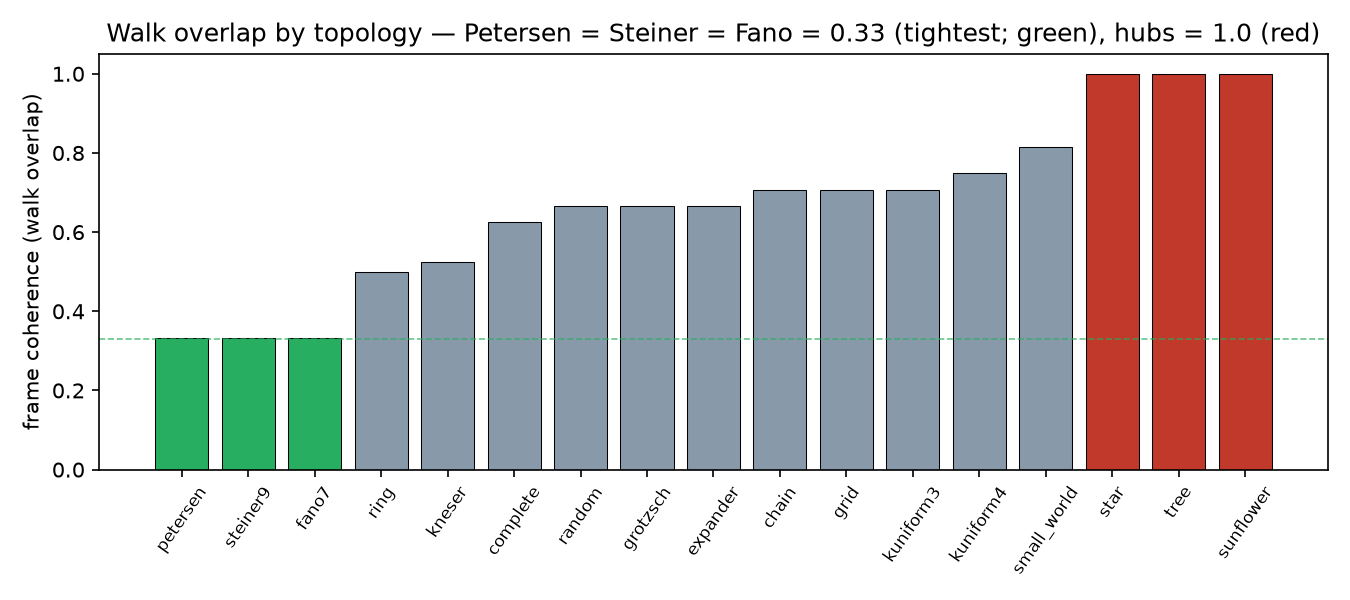
\includegraphics[width=0.9\textwidth]{figures/walk_geometry/coherence_bar.png}
\caption{Walk overlap (frame coherence) by topology, sorted.}\end{figure}

\section{Use, and one caveat}
The zoo feeds \texttt{controller\_bench}: each topology becomes a learned HSiKAN controller fitting each plant.
Invariants are the regressors. \textbf{One result already in hand (companion note for Kati):} frame coherence
does \emph{not} rank control --- the matched (isomorphic) controller wins per plant, not the lowest-coherence one.
So the zoo's value is as the \emph{family} over which the matching law is measured, not a ranking of ``best''
topologies. Code: \texttt{hymeko\_rl/\{topology\_zoo,\,topology\_invariants,\,hypergraph\_designs,\,controller\_bench\}.py};
tests under \texttt{hymeko\_rl/tests/}.
\end{document}
